\chapter{Final Design}
\label{chap:detailed_design}

This chapter presents the final design process for the rotating climbing wall, focusing on the key subsystems, as well as the integration of these systems. Each main component was selected and designed to meet the requirements set out in Chapter \ref{chap:concept_design}. Structural verification was carried out through both analytical and simulation-based approaches.

Due to the complex nature of verifying stress and displacement in many of the mechanical systems, the native Finite Element Method (FEM) package in Autodesk Fusion 360 was employed to perform static simulations. To ensure the correct usage of the package, a verification process was conducted (as detailed in Appendix~\ref{appx:FEM-verification}). A simulation was performed on a simple test case, where the FEM package overestimated stress by just over 5\% and displacement within 0.6\%. These results provided confidence to utilize the package for more complex simulations.

\section{Main Dimensions}

As discussed in the technology review (see Chapter~\ref{chap:technology_review}), typical market products for rotating climbing walls vary in size. The largest, the Treadwall Max6/12, features a climbing surface measuring 1.83\,m in width and 3.1\,m in height, while the smallest, the Treadwall Kore4/11, measures 1.22\,m in width and 2.75\,m in height.

For this design, a middle ground was chosen, with dimensions of approximately 1.6\,m in width and 2.9\,m in height. This size ensures that the wall is not so small that it becomes ineffective for training or unsuitable for taller climbers, yet not so large that it significantly increases the development cost of the prototype.

All major components of the design—including shaft widths, upright beams, crossbeams, and other structural elements—were guided by these chosen dimensions.

\section{Inclination Adjustment System}

The inclination adjustment system employs a compound gear reduction mechanism to achieve precise control over the tilting angle of the climbing wall. The primary reduction stage consists of two large sector gears (curved racks) secured to the base frame and two small pinions mounted on the ends of the tilting shaft. This shaft is connected to the tilting frame via bearings and brackets to ensure smooth rotation. The torque required to drive the pinions along the sector gears is generated by a custom-designed worm gear assembly, actuated by a stepper motor. This worm gear assembly is affixed to the lower crossbeam of the tilting frame.

\subsection{Sector Gear and Pinion Design}

The sector gears have a pitch radius of 852\,mm, measured from the pivot point of the tilting mechanism. This dimension was selected based on the placement of the lower crossbeam and the worm gear assembly. The pinion gears have a pitch radius of 24\,mm, optimizing the gear ratio to enhance torque transmission while ensuring proper meshing with the sector gears.

Both the sector gears and pinions are fabricated via laser cutting from 6\,mm mild steel, chosen for its stiffness and manufacturability. Initially, the gear teeth were designed to oriented on the upper edge of the sector gears; however, they were repositioned to the lower edge to improve safety by reducing the risk of foreign objects becoming caught in the gear mesh.\\

The sector gears are securely mounted to the main frame, which has been designed for structural stability (wide legs to avoid tipping). This configuration permits a broader range of tilt angles, from $-46^\circ$ to $+30^\circ$, exceeding the requirements PR2 and PR3 specified in Section~\ref{tab:performance-requirements}. The extended range was achieved without incurring significant additional complexity or costs.\\

Given the critical role of the pinions in torque transmission, stress calculations were performed (see Appendix~\ref{calcs:pinion-SF}) to verify their structural integrity under load. Using the Lewis equation for gear tooth bending stress from \cite{budynas2015shigley}, the estimated bending stress was calculated to be 5.83\,MPa. This results in a safety factor of 42.88, based on the yield strength of the material. These results demonstrate that the pinions operate well within the acceptable stress limits, ensuring reliable performance under operational loads.


\begin{figure}[H]
    \centering
    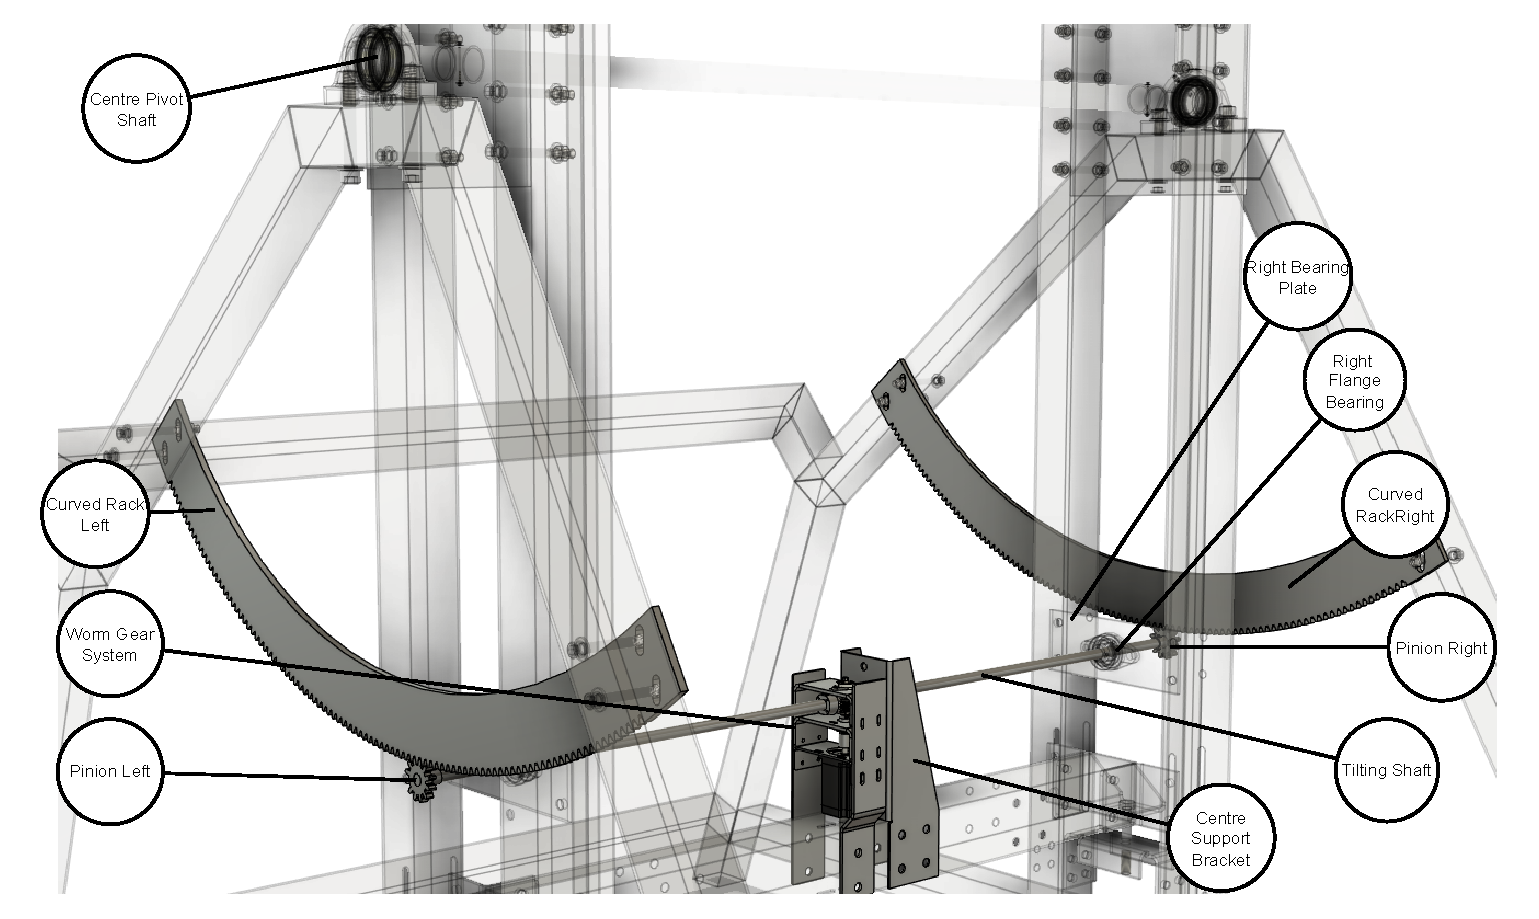
\includegraphics[width=1\linewidth]{figs/final_design/Incline_subsystem_CAD-1.pdf}
    \caption{Sector Gear and Pinion Final Design CAD Representation}
    \label{fig:sector-gear-pinion-cad}
\end{figure}

\subsection{Worm Gear Drive Assembly}

The worm gear drive assembly must be engineered to withstand substantial loads, as it maintains the entire system at the desired incline angle during operation. A mild steel shaft of 8mm thickness was chosen to transfer the torque from the stepper motor to the worm motor. The assembly comprises four critical components that must be robustly designed to prevent failure:

\begin{enumerate}
    \item \textbf{Worm Gear Set:} Converts rotational motion from the stepper motor into the torque required to drive the tilting mechanism.
    \item \textbf{Thrust Bearings:} Transfer axial force from worm gear to mounting brackets, taking axial force from pillow block bearings.
    \item \textbf{Mounting Brackets:} Secure the worm gear assembly to the tilting frame and ensure alignment of the components.
    \item \textbf{Stepper Motor:} Provides the necessary rotational input to the worm gear for inclination adjustment.
\end{enumerate}

\subsubsection{Worm Gear Set}

The worm gear set consists of a stainless steel worm (helical screw) and a brass worm wheel (helical gear). Ideally a more durable material would have been selected instead of brass, but the set was the only available worm set found that met the sizing specifications. The worm, coupled to a secondary shaft which is coupled to the stepper motor via flexible coupling, engages with the worm wheel, achieving a 28:1 reduction ratio and exhibiting self-locking properties. This design ensures that the system remains stationary when not being adjusted, providing safety and stability. The self-locking feature is critical, as it prevents back-driving, ensuring that the inclination angle remains fixed under load without the need for additional braking mechanisms. The brass worm wheel was identified as the critical component in this system and calculations were performed (see Appendix \ref{calcs:incline-system}) with a resulting gear tooth stress of 34.5MPa and safety factor of 1.3 which is slightly low, but acceptable for a prototype.

\subsubsection{Thrust Bearings}
8mm thrust bearings were selected to take the axial load of the worm gear and transfer it straight into the mounting brackets and not the shaft. The calculations performed in Appendix \ref{calcs:incline-system} yield maximum estimated force of 1.75KN with a safety factor of 1.7.


\subsubsection{Mounting Brackets}

The mounting brackets are laser-cut and bent mild steel for their relatively low price and high strength, as well as ease of manufacturing. These brackets ensure proper alignment of the worm and worm wheel and secure the assembly to the lower crossbeam of the tilting frame. Slots were designed instead of holes to allow for further alignment of the assembly. Figure \ref{fig:FEM-incline-brackets} shows the Finite Element Analysis (FEA) was performed to validate the structural integrity of the brackets under operational loads, safety factor of 1.2 (refer to Appendix~\ref{calcs:worm-bracket-fem}).

\begin{figure}[H]
    \centering
    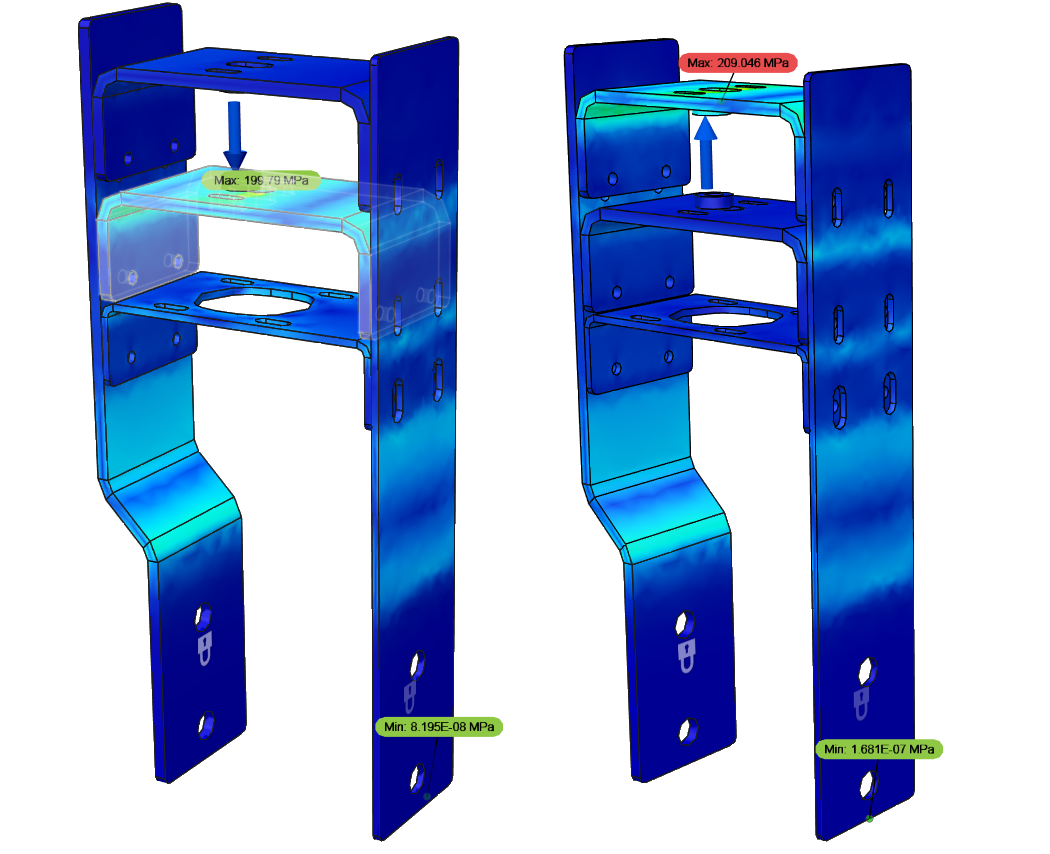
\includegraphics[width=0.6\linewidth]{figs/FEM/incline-braket.png}
    \caption{FEM Analysis Results on Worm Gear Bracket System}
    \label{fig:FEM-incline-brackets}
\end{figure}

\subsubsection{Stepper Motor Selection}
To determine the appropriate motor for driving the inclination adjustment system, calculations were performed (see Appendix~\ref{calcs:stepper-motor}) to establish the required torque and speed. The torque required was calculated to be 1.87\,Nm, while speed was not a critical factor since tilt speed was not specified as a requirement. 

A Nema 23 stepper motor, with an output torque of 2\,Nm, was selected as it met the torque requirements. Additionally, it was available in stock at the mechatronics store, and stepper motors are both cost-effective and offer precise control, making it an ideal choice for this application.

\subsection{Shaft Selection}
Following FEM simulations (see Appendix~\ref{calcs:incline-system}) that used the maximum expected torque on the shaft as input (from Section~\ref{calcs:incline-system}), a 16\,mm mild steel shaft was selected. The analysis showed a safety factor of 1.54 and a displacement of 0.746\,mm under the given load which were deemed acceptable for the prototype.

The shaft is supported by three UCFL203FKD/ISO flange bearings, chosen for their size and affordability. Since the bearings were considered non-critical components, it was assumed they could sufficiently handle the expected loads without failure.


\begin{figure}[H]
    \centering
    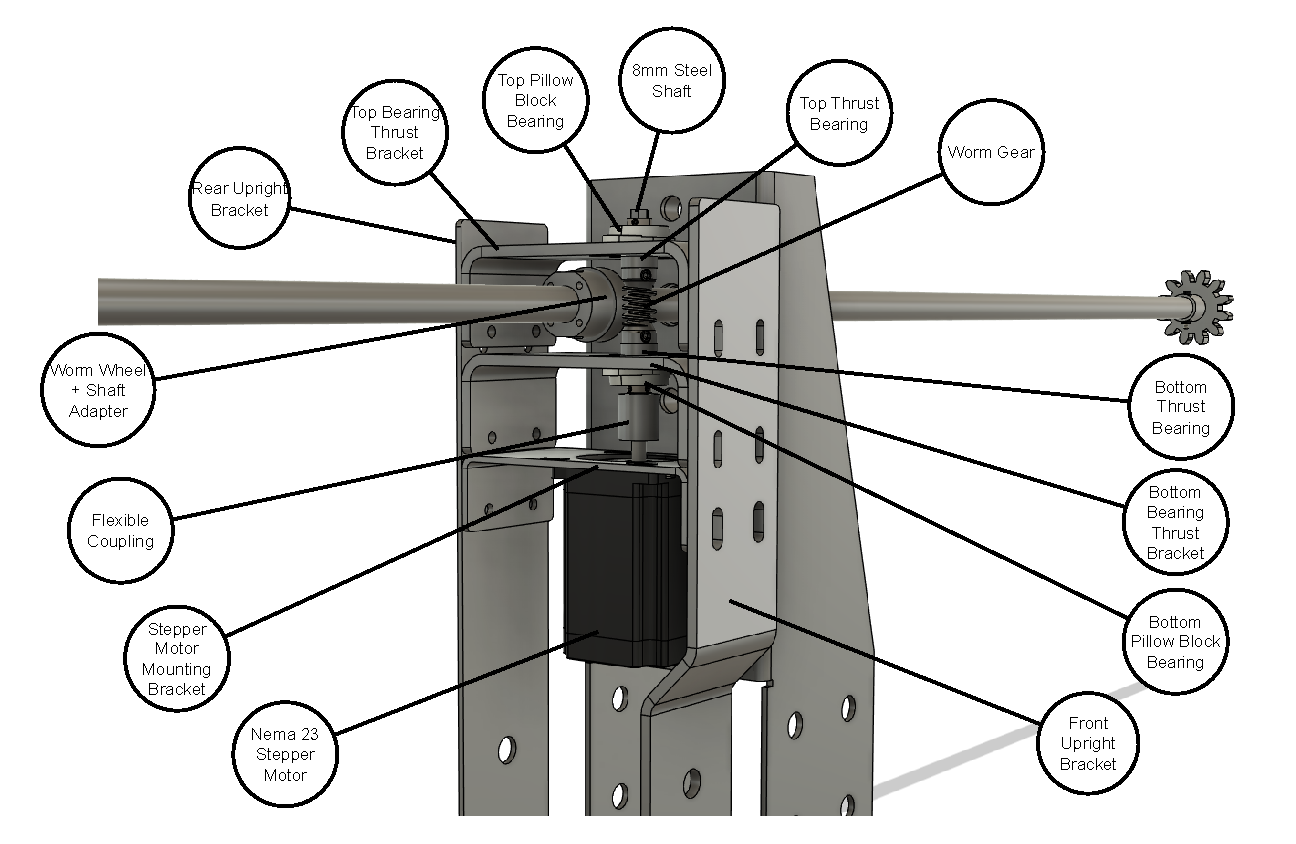
\includegraphics[width=1\linewidth]{figs/final_design/wormgear_assembly_CAD.pdf}
    \caption{Worm Gear Drive Assembly Final Design CAD Representation}
    \label{fig:worm-gear-drive-cad}
\end{figure}


\section{Braking System}

The braking system was designed to include an active braking component secured to the top crossbeam. Due to space limitations, the bottom crossbeam was reserved for the tilting system, necessitating the placement of the braking mechanism on the top crossbeam. This subsystem utilizes a pulley-driven AC servomotor for electromagnetic braking, with the main driven shaft mounted through a series of three deep groove flange ball bearings. These bearings are \textbf{Koyo UCF205 Flange unit bearings}, chosen for their ability to handle the calculated loads and ease of mounting. The bearings are mounted via laser-cut and bent sheet metal brackets to the top crossbeam. Figure~\ref{fig:brake-system-final-design} shows the final braking system CAD representation.

\subsection{Main Shafts}

To maintain a constant speed on the rotating surface, a braking torque of 210\,Nm was required on the top main shaft. This calculation was based on a climber’s weight estimate of 1400\,N, providing an added safety margin (excluding friction). The downward force on each sprocket of the shaft was calculated to be 1.11\,kN (calculations can be found in Appendix \ref{calcs:main_braking_shaft}).

Bright mild steel was selected as the shaft material due to its cost-effectiveness and strong mechanical properties. Finite Element Analysis (FEA) was performed in Autodesk Fusion 360 on both 30\,mm and 25\,mm diameter solid shafts, yielding safety factors of 3.47 and 2.24, respectively. Based on these results, a 25\,mm solid bright steel shaft was chosen for both the top and bottom main shafts.

Figure~\ref{fig:FEM-mainshaft} displays the FEA results for the shaft, revealing a stress concentration toward the middle. To address this, an extra Koyo UCF205 bearing was placed near the middle of the shaft to provide additional support.

\begin{figure}[h]
    \centering
    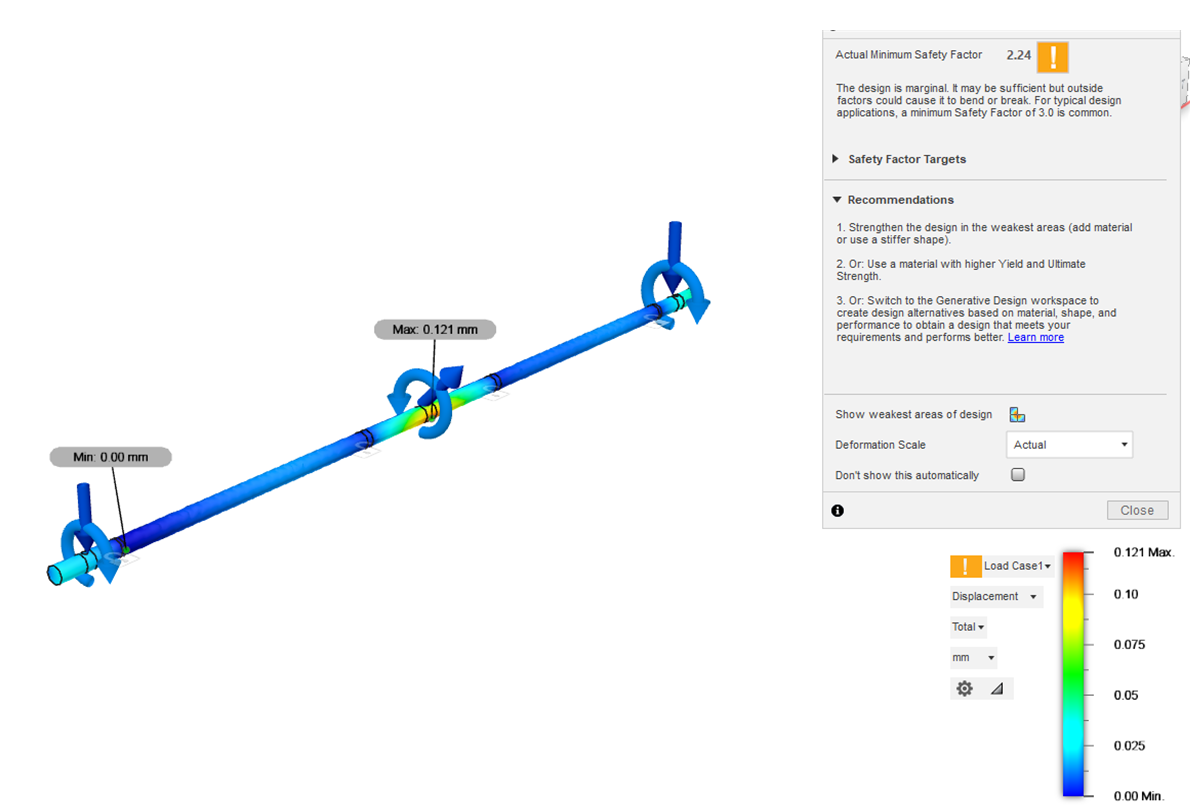
\includegraphics[width=0.8\linewidth]{figs/final_design/FEMShaft.png}
    \caption{FEA Results of 25\,mm Diameter Main Shaft}
    \label{fig:FEM-mainshaft}
\end{figure}

\subsection{Brackets and Bearings}

The brackets were designed to be laser-cut and bent from mild steel due to its favorable cost-to-strength ratio. Stainless steel was considered for its extra strength and corrosion resistance but was ruled out since the wall will be placed indoors, and mild steel can be painted to prevent rust. Due to the complexity of the bracket shapes, FEA was performed using 6\,mm thick mild steel, simulating the worst-case scenario of holding the entire weight of the climber, panels, and chain tension. The safety factor at a vertical wall inclination was 5.93, while at a $-45^\circ$ inclination, the safety factor was 1.33. Although slightly low, the high load estimate and prototype nature of the wall justify this. Figure~\ref{fig:FEM-bracket} shows the FEA results of the bracket at a $45^\circ$ incline. Further calculations can be found in Appendix \ref{calcs:brackets_bearings}.

\begin{figure}[ht]
    \centering
    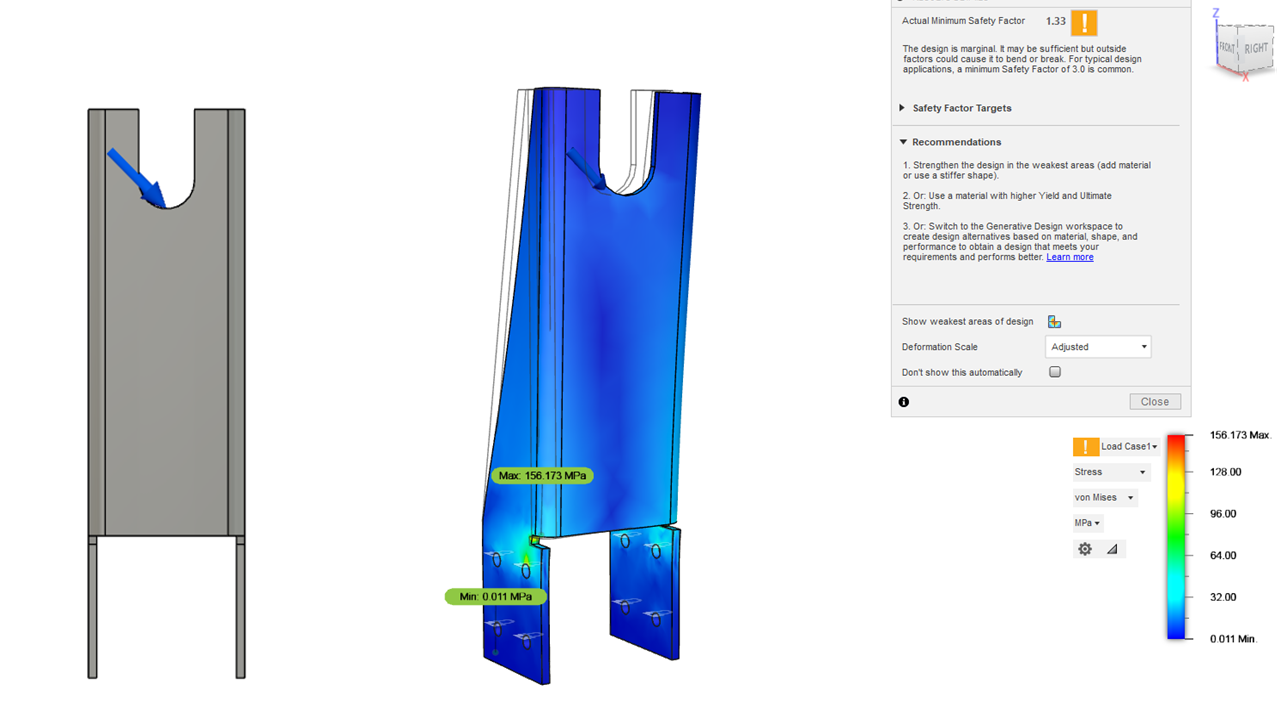
\includegraphics[width=0.8\linewidth]{figs/final_design/FEMBracket45.png}
    \caption{FEA Results of Bracket at $45^\circ$ Incline}
    \label{fig:FEM-bracket}
\end{figure}

\subsection{Motor and Belt Drive System}

The top shaft must resist approximately 50\,Nm of torque, factoring in friction losses of around 61\,Nm (for a lighter climber weight of 90\,kg). Calculations for this are found in Appendix \ref{calcs:motor_belt}. This system prioritizes cost control while maintaining sufficient safety.

An AC servomotor and driver system was selected; the \textbf{MiGE 130ST-M10010} motor was chosen for its suitable specifications (see Table~\ref{tab:motor_specs}). A basic calculation was performed to determine the necessary torque reduction ratio after accounting for mechanical losses.

\begin{table}[H]
    \centering
    \begin{tabular}{|l|c|}
        \hline
        \textbf{Motor Model} & 130ST-M10010 \\
        \hline
        Rated Power (kW) & 1.0 \\
        \hline
        Rated Voltage (V) & 220 \\
        \hline
        Rated Current (A) & 4.5 \\
        \hline
        Rated Speed (rpm) & 1000 \\
        \hline
        Holding Torque (Nm) & 10 \\
        \hline
        Peak Torque (Nm) & 20 \\
        \hline
        Voltage Constant (V/krpm) & 140 \\
        \hline
        Torque Coefficient (Nm/A) & 2.2 \\
        \hline
        Rotor Inertia (kg$\cdot$m$^2$) & $1.94 \times 10^{-3}$ \\
        \hline
        Line-Line Resistance ($\Omega$) & 2.7 \\
        \hline
        Line-Line Inductance (mH) & 8.8 \\
        \hline
        Mechanical Time Constant (ms) & 3.26 \\
        \hline
        Weight (kg) & 11.5 \\
        \hline
    \end{tabular}
    \caption{MiGE Motor Specifications}
    \label{tab:motor_specs}
\end{table}

With a peak holding torque of 20\,Nm, a continuous torque of 10\,Nm, and a power rating of 1\,kW, this motor is well-suited for the application when paired with the appropriate gear reduction system.

\subsubsection*{Torque Reduction Ratio Calculation}

The required torque at the shaft is:

\[
T_{\text{shaft}} = 45.44\ \text{Nm}
\]

The motor's continuous torque is:

\[
T_{\text{motor}} = 10\ \text{Nm}
\]

Therefore, the necessary gear reduction ratio (\( R \)) is:

\[
R = \frac{T_{\text{shaft}}}{T_{\text{motor}}} = \frac{45.44\ \text{Nm}}{10\ \text{Nm}} = 4.544
\]

A gear reduction ratio of approximately 5:1 is required to meet the torque demands. The SKF Power Transmission Belt Software \cite{SKF_BeltDriveTool} was used to select an M5 timing belt and a 90-tooth to 18-tooth pulley system, providing the needed 5:1 gear ratio. This results in a continuous torque of 50\,Nm and a maximum torque of 100\,Nm on the main shaft, meeting the main shaft torque and speed criteria. Belt calculations are found in Appendix \ref{calcs:motor_belt}.

\subsection{Braking Resistor}

To dissipate the energy generated by the motor due to the climber's weight and resulting rotation, a braking resistor is employed. The resistor is connected to the designated output pins on the motor driver, with the required values calculated in Appendix \ref{calcs:braking_resistor}. Finding a braking resistor with exactly these specifications is challenging, so the braking resistor that was purchased was overspecified. Table~\ref{tab:braking-resistor-specs} shows the calculated values and the specifications of the selected resistor.

\begin{table}[H]
    \centering
    \begin{tabular}{|l|c|c|}
        \hline
        \textbf{Specification} & \textbf{Calculated Value} & \textbf{Selected Resistor Value} \\
        \hline
        Power (W) & 227.2 & 1000 \\
        \hline
        Resistance ($\Omega$) & 2.19 & 16 \\
        \hline
    \end{tabular}
    \caption{Braking Resistor Specifications}
    \label{tab:braking-resistor-specs}
\end{table}

Figure~\ref{fig:brake-system-final-design} illustrates the final CAD design of the braking system.

\begin{figure}[H]
    \centering
    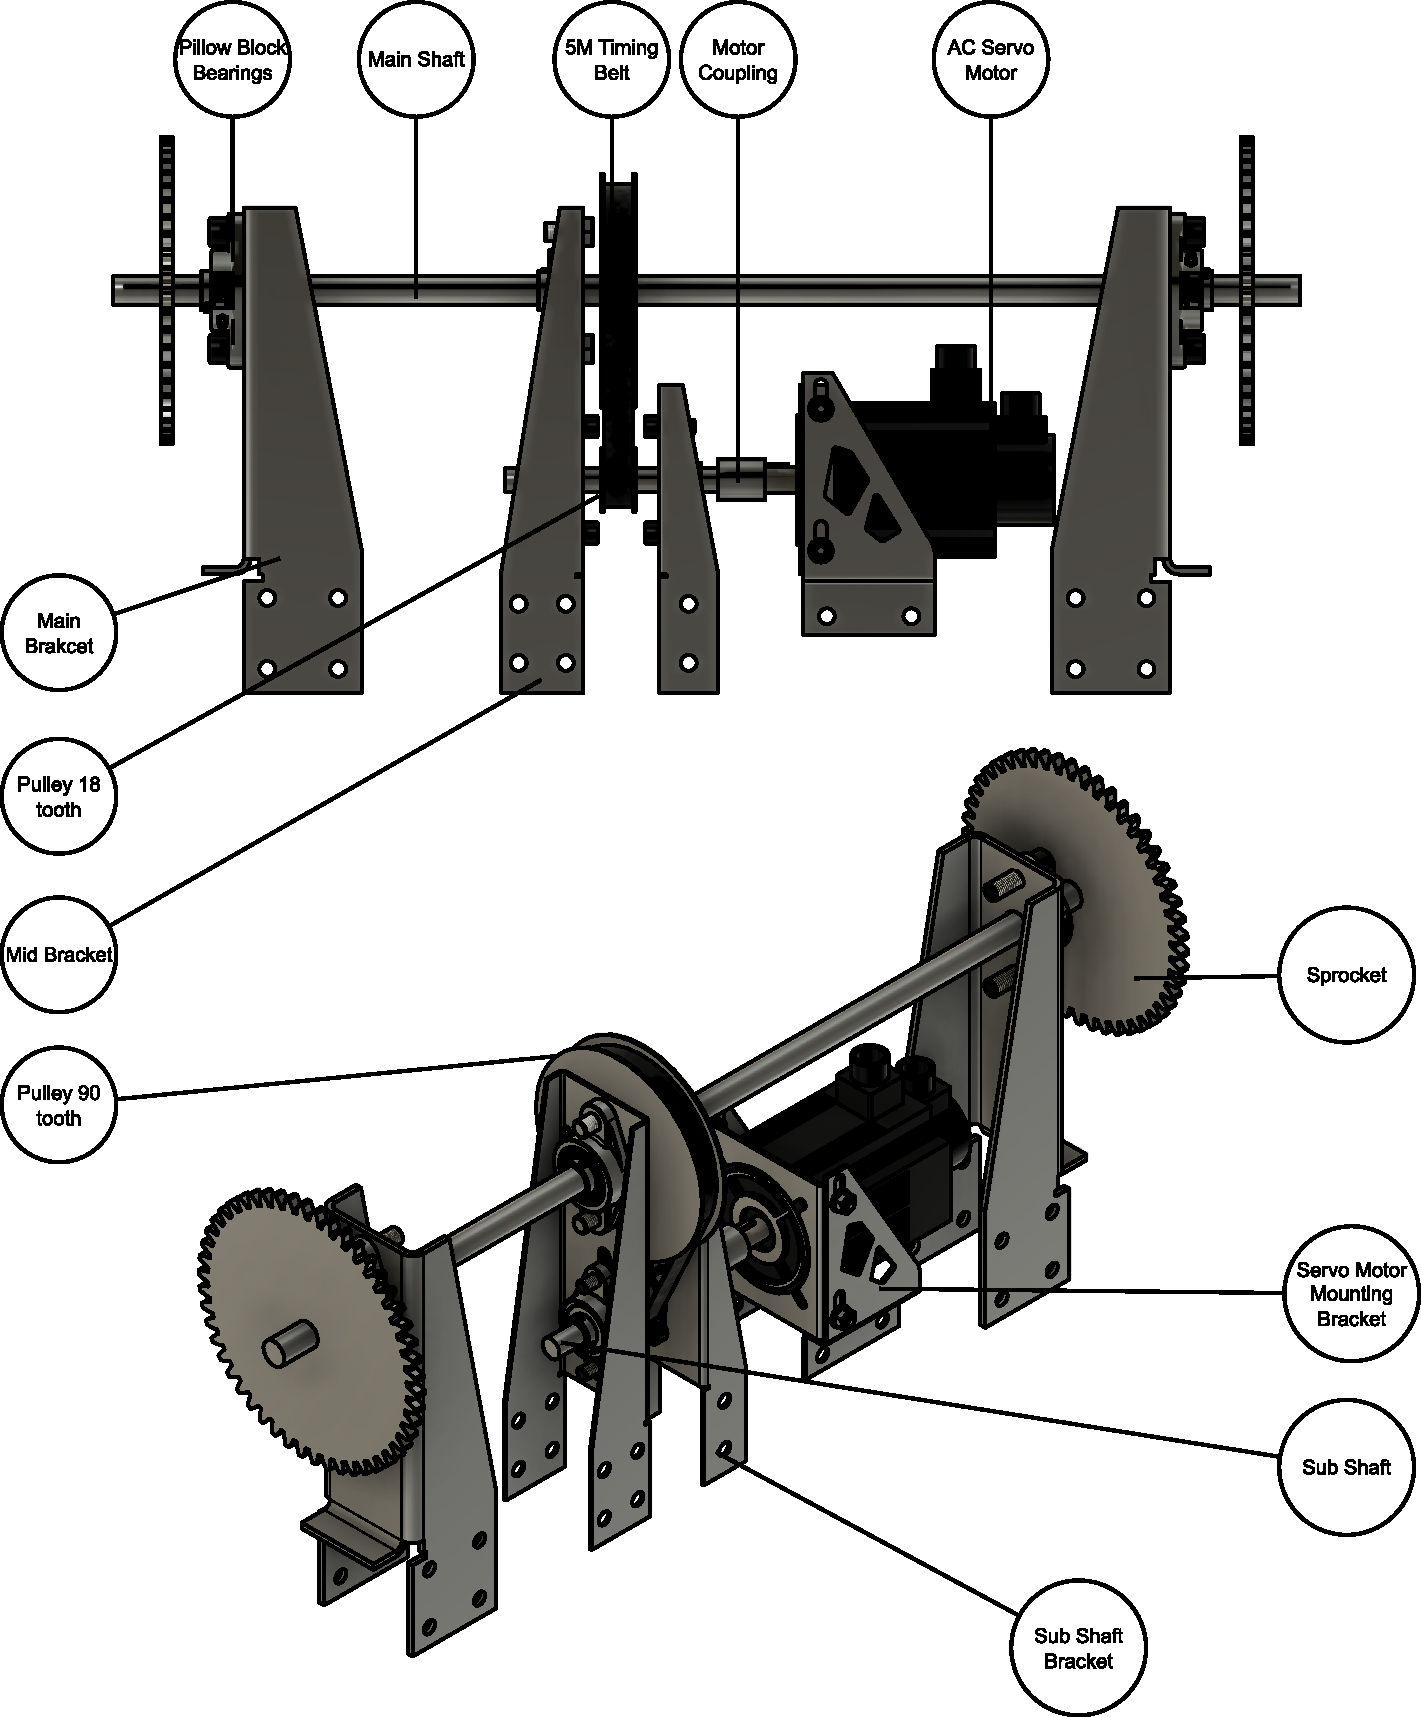
\includegraphics[width=0.8\linewidth]{figs/final_design/BrakingSyst.pdf}
    \caption{Braking System Final CAD Design}
    \label{fig:brake-system-final-design}
\end{figure}

\section{Final Assembly}

The final CAD assembly is shown below, though the main components are shielded by panels. Additional renders with panels removed will be included in the final report. The chain has been selected but is yet to be added to the CAD model.

\begin{figure}[ht]
    \centering
    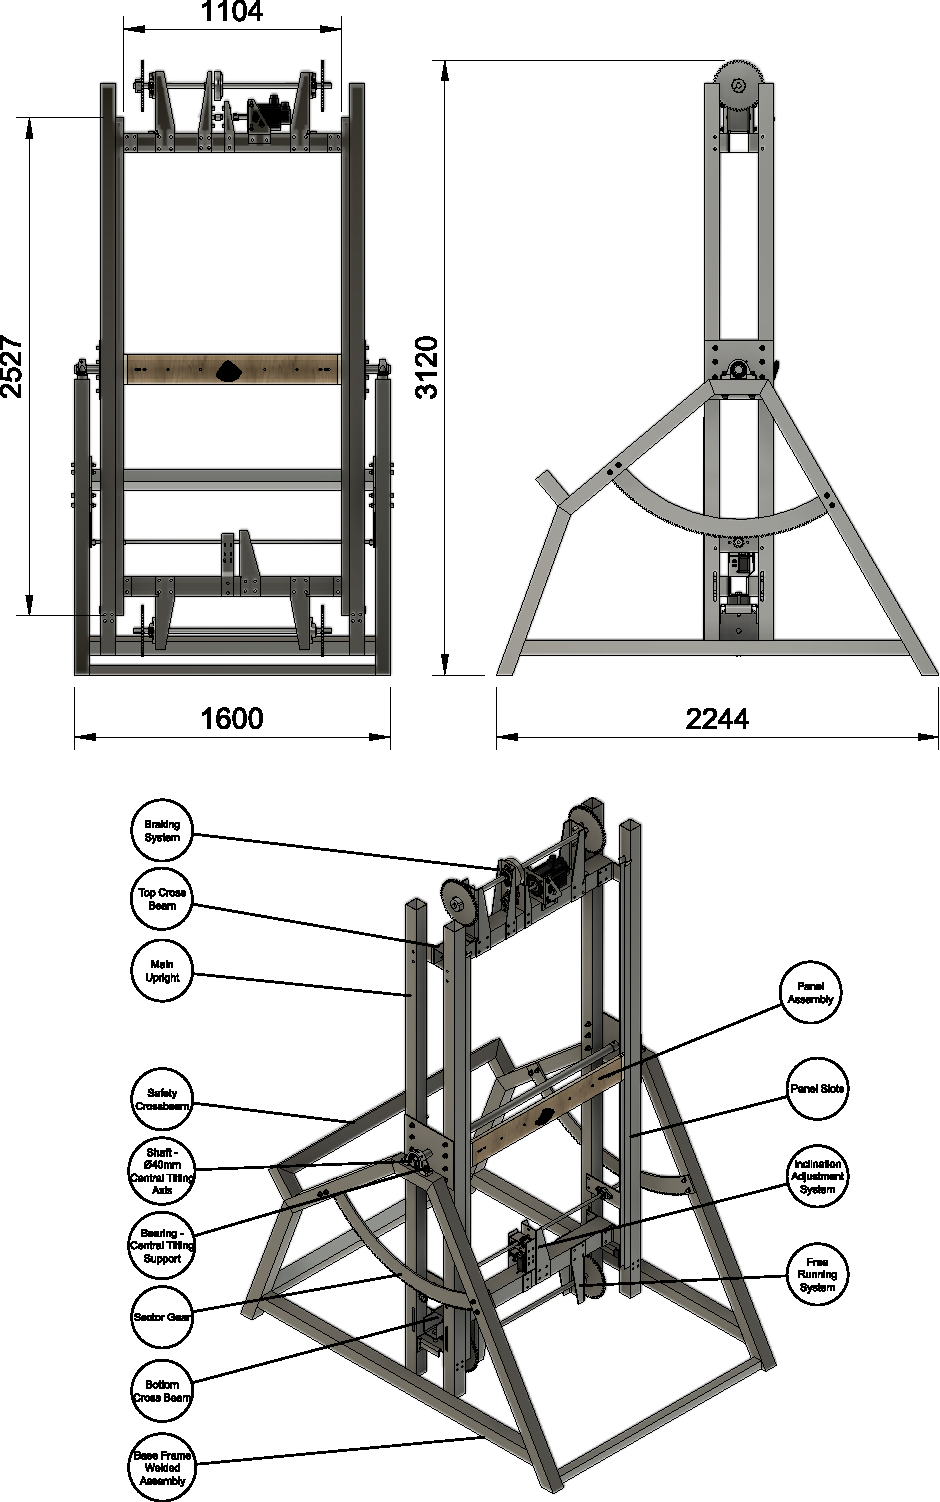
\includegraphics[width=1.0\linewidth]{figs/final_design/Main_Assembly_CAD.pdf}
    \caption{Full Assembly Final CAD Design}
    \label{fig:full-assembly-final-design}
\end{figure}
